\documentclass[a4paper]{article}

\usepackage[utf8]{inputenc}
\usepackage[portuguese]{babel}
\usepackage{a4wide}
\usepackage[pdftex]{hyperref}
\usepackage{graphicx}
\usepackage{wrapfig}
\usepackage{amsmath}
\usepackage{verbatim}
\usepackage{caption}
\usepackage{subcaption}
\usepackage{float}
\usepackage{blochsphere}
\usepackage{amsfonts}


\begin{document}

\begin{titlepage}
\begin{center}



\includegraphics[width=0.4\textwidth]{logo.jpg}\\[0.5cm]

\vspace{10mm}

{\huge Universidade do Minho - Escola de Engenharia}\\[0.5cm]

{\large Relatório do trabalho prático de Computação Gráfica}\\[0.5cm]

\vspace{10mm} 

% Title
\rule{\linewidth}{0.5mm} \\[0.4cm]
{ \huge \bfseries Fase 1 – Primitivas Gráficas \\[0.4cm] }
\rule{\linewidth}{0.5mm} \\[1.5cm]

% Author and supervisor
\noindent
\begin{minipage}{0.4\textwidth}
  \begin{flushleft} \large
    \emph{Autores :}\\
    Daniel Maia \textsc{(A77531)}\\
    
\includegraphics[width=1.5cm]{daniel.jpg}\break
    Diogo Silva\textsc{(A78034)}\\
    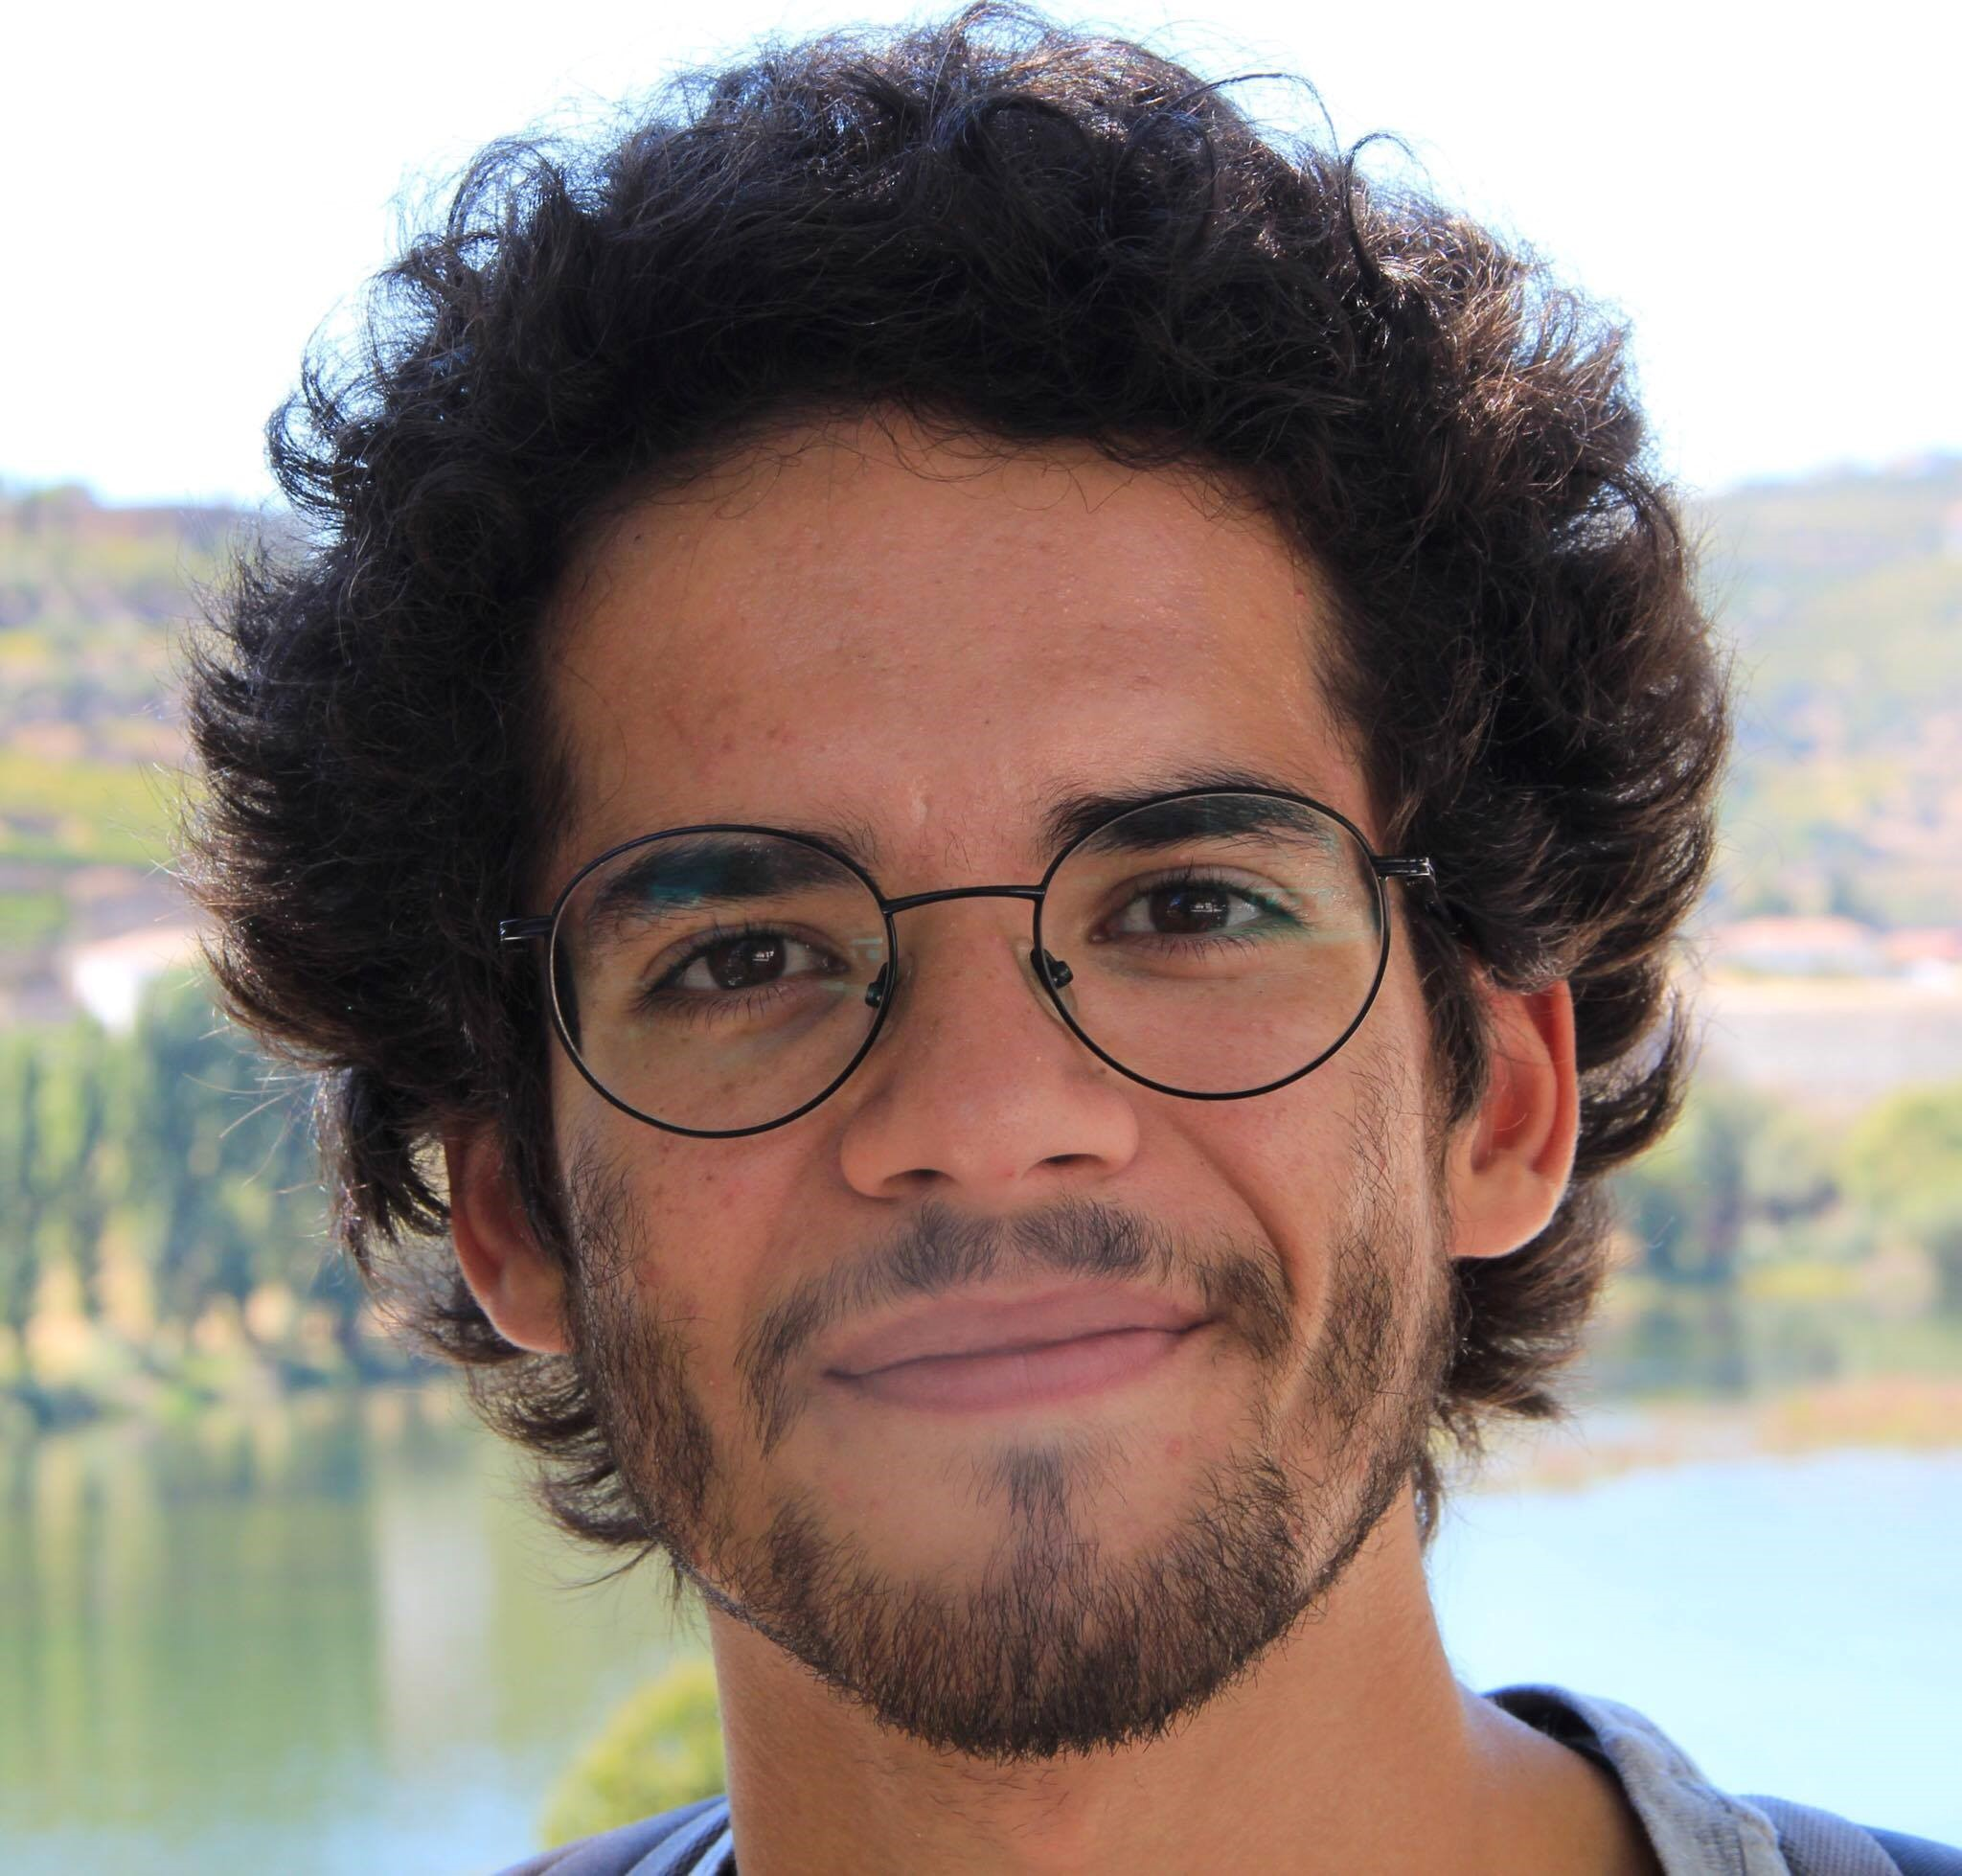
\includegraphics[width=1.5cm]{afonso.jpg}\break
    Marco Silva\textsc{(A79607)}\\
    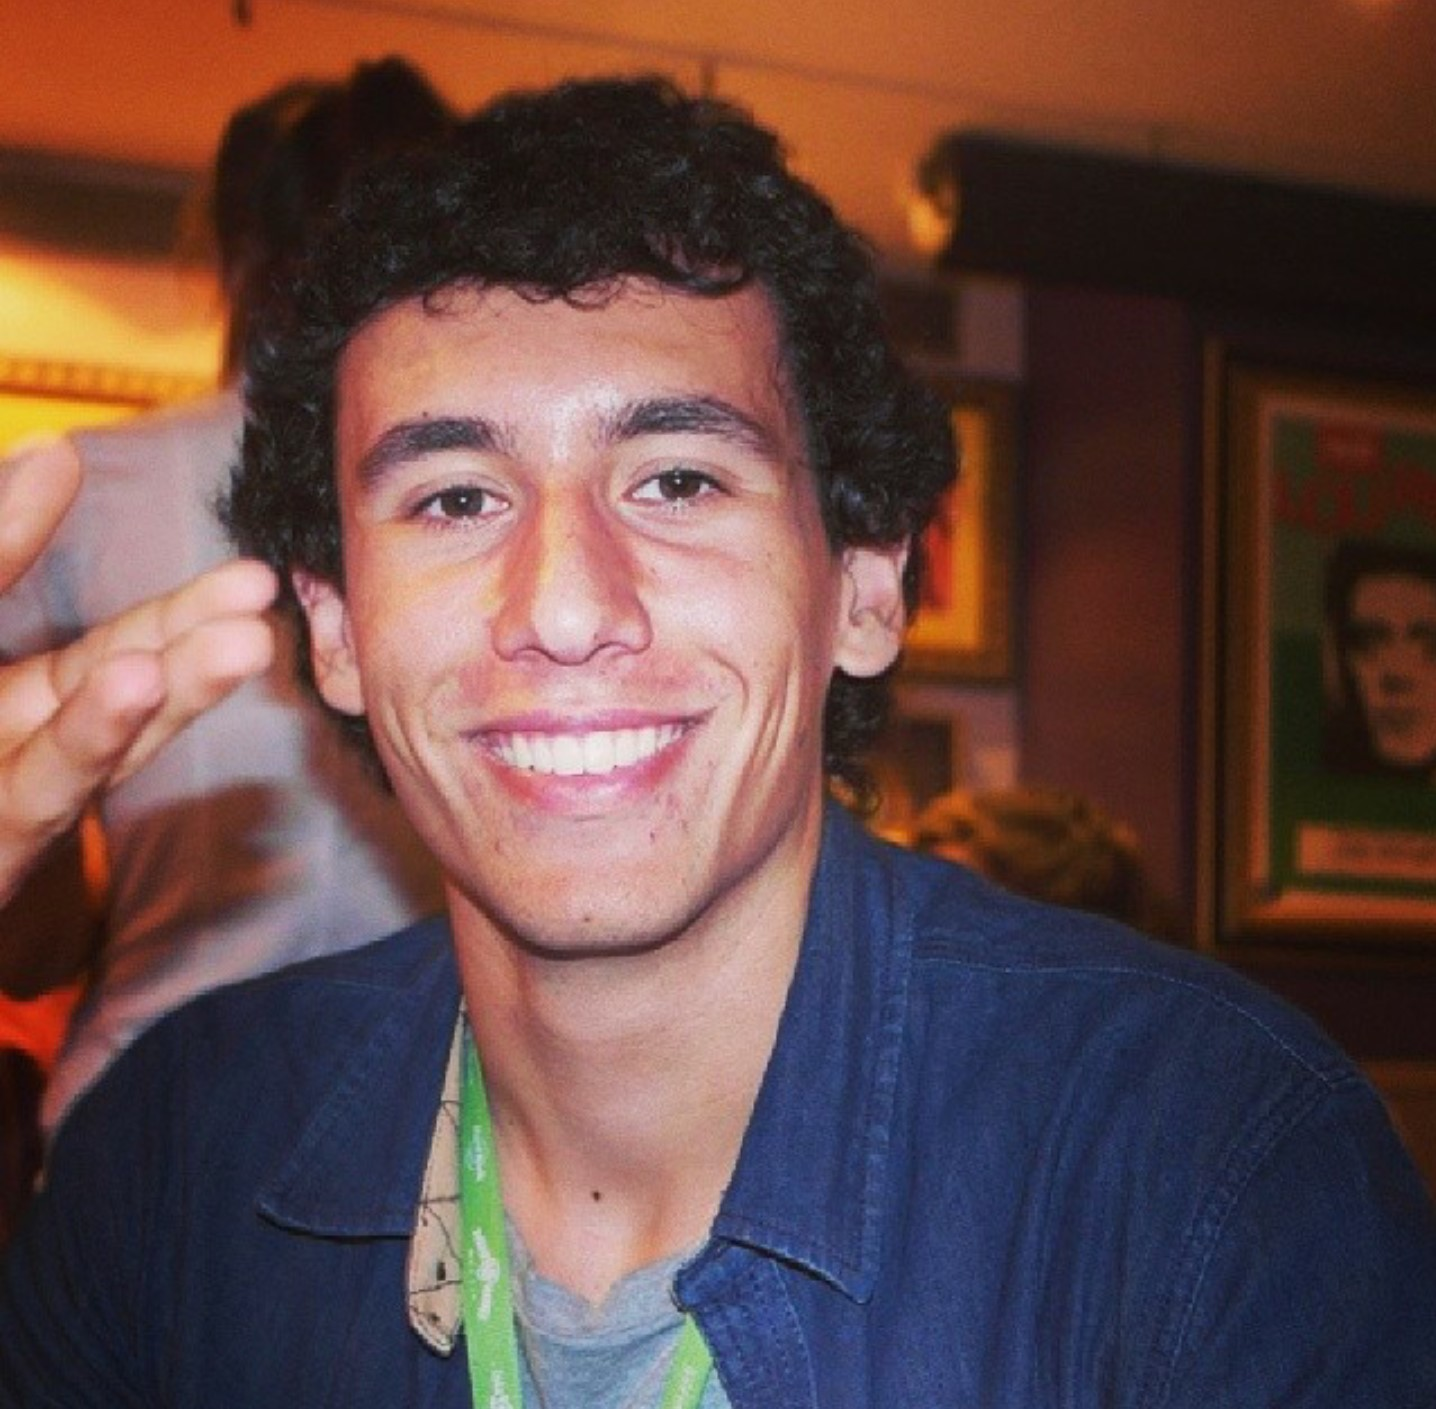
\includegraphics[width=1.5cm]{marco.jpg}\break
  \end{flushleft}
\end{minipage}%
\vfill

% Bottom of the page
{\large Versão 1.0 \\ \today}

\end{center}
\end{titlepage}


\begin{abstract}%DANIEL

\hspace{3mm} O objetivo desta fase do trabalho prático é criar cenas hierárquicas em XML recorrendo a transformações geométricas. Uma cena é definida por uma árvore cujos nodos contêm um conjunto de transformações geométricas, nomeadamente, \textit{translate, rotate} e \textit{scale}, e, opcionalmente, um conjunto de modelos. Cada poderá ter também um ou mais filhos. 

\par Para demonstrar o resultado do trabalho nesta fase, definir-se-á também uma cena com o modelo estático do sistema solar, com o Sol, os planetas e luas, definidos numa hierarquia.

\end{abstract}

\pagebreak
\tableofcontents

\pagebreak

% ===================================================
\section{Introdução}%DANIEL

\hspace{3mm} Tendo na fase anterior sido construídas uma aplicação \textit{generator}, que cria modelos primitivos de figuras, e uma aplicação \textit{engine}, capaz de demonstrar as figuras referidas através de um ficheiro de configuração em XML, proceder-se-á ao desenvolvimento de funcionalidades do \textit{engine}. Inicialmente, este teve apenas a capacidade de desenhar primitivas no ecrã exatamente como foram definidas pelo \textit{generator}. Como se pretende utilizar este programa para renderizar cenas, será necessário que este consiga efetuar \textbf{transformações geométricas}.

\par Uma transformação geométrica define-se como uma função que altera as propriedades de um ou mais eixos de coordenadas, geralmente em $\mathbb{R}^2$ ou $\mathbb{R}^3$. Através destas, é possível desenhar figuras mais complexas a partir de primitivas simples. Para este projeto, focou-se especificamente em três:  

\begin{itemize}
    \item Translações, que movem a origem do sistema de coordenadas por um vetor de coordenadas \texttt{(u,v,w)};
    \item Rotações, que rodam um ou mais eixos de coordenadas no sentido anti-horário à volta de um ângulo $\alpha$;
    \item Escalas, que aumentam ou diminuem a distância entre unidades de comprimento de um ou mais eixos do sistema de coordenadas.
\end{itemize}

\par Uma \textbf{cena} define-se como uma árvore cujos nodos contêm um conjunto das transformações geométricas descritas, bem como, opcionalmente, um conjunto de modelos primitivos e um grupo de nodos filho. Qualquer nodo filho herdará as transformações aplicadas ao respetivo pai. Transformações geométricas existem exclusivamente dentro de um grupo e são aplicadas a todos os modelos e subgrupos.

\par Tendo atualizado as capacidades do \textit{engine}, proceder-se-á ao desenvolvimento de um ficheiro XML que descreva um modelo do nosso Sistema Solar para demonstrar o funcionamento do programa. É de notar que as primitivas utilizadas pelo ficheiro XML em questão serão criadas pela aplicação \textit{generator} existente.

% ===================================================
\section{Descrição do Trabalho e Análise de Resultados}

\subsection{Sistema solar em \emph{XML}} 

% Falar da estrutura do XML [MARCO]
\subsubsection{Estrutura do \emph{XML}}

\hspace{3mm} A descrição do sistema solar será feita através de um ficheiro \emph{XML}. Este ficheiro, encontra-se estruturado sob a forma de uma árvore em que cada um dos seus nodos poderá conter um conjuntos de transformações e um ou mais modelos que devem ser representados. Estes modelos são os ficheiros .3d gerados pelo \emph{generator} que contêm a representação das formas a desenhar sobre a forma de pontos.

\par Teremos então como possibilidade nodos do tipo \emph{group} e \emph{models}. Tem-se ainda o nodo \emph{scene} que constituirá a árvore de representação de uma cena completa. Em qualquer um dos tipos de nodos podem também ser definidos novos nodos, também designados por nodos filhos. Todas as transformações definidas em nodos de nível acima na árvore do ficheiro deverão ter efeito em nodos de maior profundidade e consequentemente, o efeito de qualquer transformação não se deve propagar para grupos de profundidade inferior na árvore de representação da cena. Estas transformações apenas podem existir dentro de nodos do tipo \emph{group} e estas devem ser consideradas apenas dentro do mesmo. De salientar ainda que, a ordem pela qual as transformações são definidas terá de ser considerada no momento do desenho da cena.

% Falar da pesquisa feita [DANIEL]
\subsubsection{O Sistema Solar}



% Falar da hierarquia usada para representar o sistema solar [MARCO]
\subsubsection{Hierarquia do Sistema Solar}

\hspace{3mm} Tendo em conta a estruturação do ficheiro \emph{XML} definida mais a cima neste relatório, o sistema solar encontra-se representado em apenas uma cena, constituida por vários grupos.

\par Para que a interpretação do ficheiro de representação do sistema solar fosse o mais direta possível, os elementos constituintes do mesmo foram definidos começando no centro pelo Sole finalmente, so restantes planetas e respetivas luas, começando pelos que se encontram mais próximos do Sol e terminando nos mais longínquos.

\par Para cada um destes, foi definido um nodo do tipo \emph{group} de modo a que fosse possível definir para representação para além do planeta em si, outros elementos considerados relevantes tais como luas ou satélites.


% Falar do resultado final [MARCO]
\subsubsection{Resultado Final}


% ---------------------------------------------------

\subsection{Carregamento do XML} %[AFONSO]
% Que biblioteca é usada
% Estrutura de dados usada para armazenar a info
% Como é feito? Iteradores + atof
% Quando é que é feito?
% Vantagens de ter a estrutura de dados em vez de ler sempre do ficheiro



% ---------------------------------------------------

\subsection{Construção da cena} %[AFONSO]
% Como é desenhada? drawGroup + PushMatrix + PopMatrix
% Quando é desenhada? PostRedisplay...


\newpage
% ===================================================
\section{Conclusões e Sugestões}



\newpage
% =========================================================
\bibliographystyle{unsrt}
\bibliography{biblio}


\end{document}
